\documentclass[tikz, border=12pt]{standalone}
\usepackage[utf8]{inputenc}
\usepackage[T5]{fontenc}
\usepackage{lmodern}
\usepackage{xcolor}
\usepackage{graphicx}
\usetikzlibrary{positioning, calc, arrows}

\begin{document}
\begin{tikzpicture}[
  >=stealth,
  font=\sffamily,
  % Container style: Khung nét đứt màu đen thanh mảnh trên nền trắng tinh
  dashedContainer/.style={
    draw=black,
    dashed,
    line width=1.0pt,
    fill=white,
    rounded corners=5pt,
    inner sep=8pt,
    align=center
  },
  % Sub-box style
  innerDashed/.style={
    draw=black!80,
    dashed,
    line width=0.8pt,
    fill=white,
    rounded corners=3pt,
    align=center,
    inner sep=4pt
  },
  % Mũi tên đen thanh mảnh
  arrowLine/.style={
    ->,
    line width=1.2pt,
    draw=black
  },
  biArrowLine/.style={
    <->,
    line width=1.2pt,
    draw=black
  },
  % Nhãn trên mũi tên tối giản
  tagText/.style={
    font=\small\bfseries,
    fill=white,
    inner sep=2.5pt,
    text=black
  }
]

% ==================== TẦNG 1: TẦNG ĐEO ====================
\node[dashedContainer, text width=15.0cm] (t1) at (0, 0) {
  \begin{tikzpicture}
    % Tiêu đề góc trái
    \node[anchor=west, font=\bfseries\normalsize] at (-7.2, 1.4) {Tầng đeo (Wearable Tier)};
    
    % Hình 1: Khung nẹp 3 ngón
    \node (img_splint) at (-4.2, 0) {
      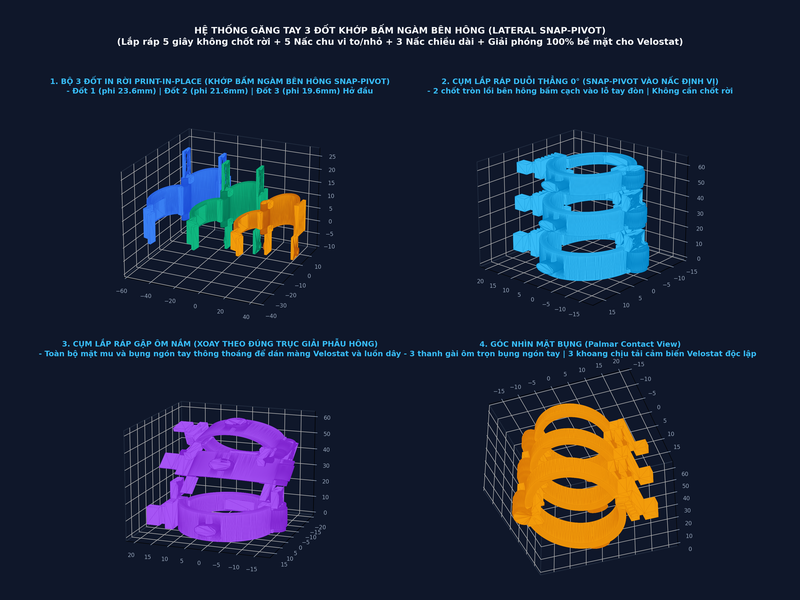
\includegraphics[width=4.0cm, height=2.2cm, keepaspectratio]{assets/splint_3d.png}
    };
    \node[below=2pt of img_splint, font=\footnotesize] {Khung nẹp 3 ngón in 3D};
    
    % Mũi tên nhỏ liên kết trong nẹp
    \draw[arrowLine] (-1.8, 0) -- (-0.8, 0);

    % Hình 2: Cảm biến vi sai & Ngàm bản lề
    \node (img_mech) at (1.5, 0) {
      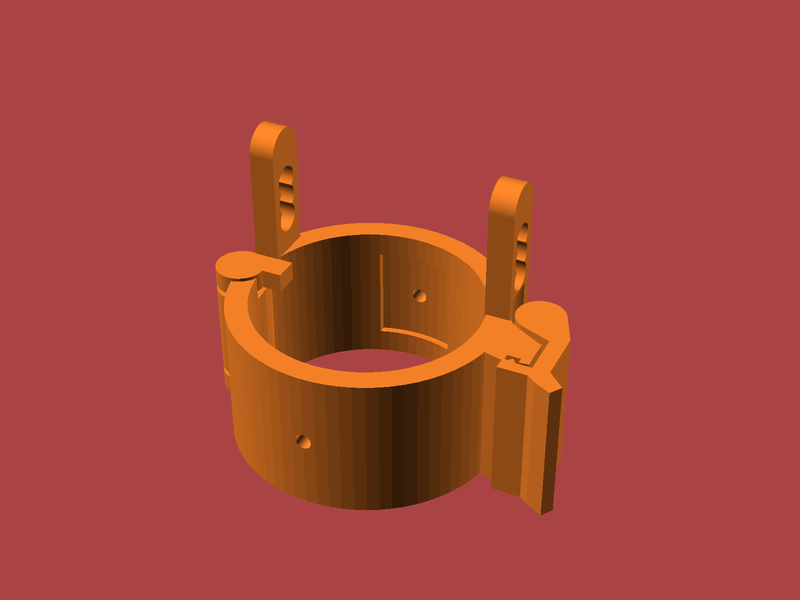
\includegraphics[width=4.0cm, height=2.2cm, keepaspectratio]{assets/mech9.png}
    };
    \node[below=2pt of img_mech, font=\footnotesize] {16 Ô Velostat vi sai + 3 Flex};

    % Nhãn chú thích bên phải
    \node[anchor=west, align=left, font=\scriptsize] at (4.0, 0) {
      $\bullet$ Khóa ngàm 2 bản lề đóng 1 tay\\
      $\bullet$ Đo lực tiếp xúc \& góc uốn\\
      $\bullet$ Chốt mở nhanh tháo khẩn cấp
    };
  \end{tikzpicture}
};

% ==================== TẦNG 2: TẦNG THU THẬP & DSP ====================
\node[dashedContainer, text width=15.0cm, below=28pt of t1] (t2) {
  \begin{tikzpicture}
    \node[anchor=west, font=\bfseries\normalsize] at (-7.2, 1.4) {Tầng thu thập \& Xử lý DSP (Sensing \& DSP Tier)};
    
    % Box ESP32-S3
    \node[innerDashed, text width=5.2cm] (b_esp) at (-4.2, 0) {
      {\bfseries\small ESP32-S3 + ADS1115 (16-bit)}\\[2pt]
      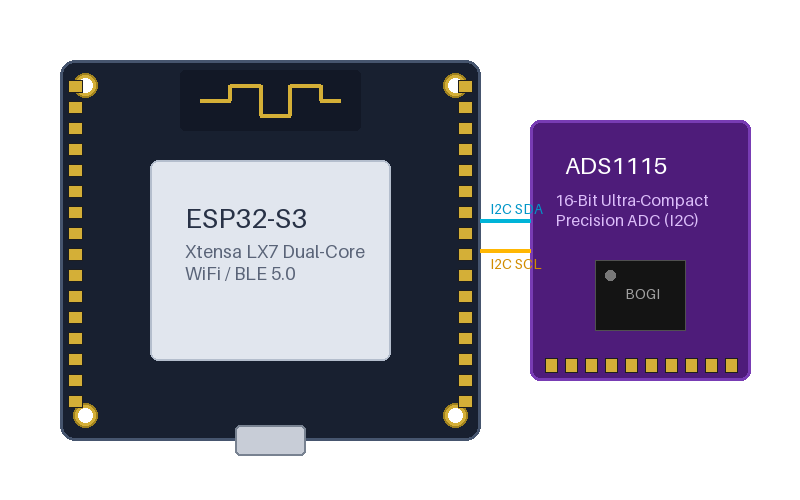
\includegraphics[width=4.8cm, height=1.9cm, keepaspectratio]{assets/controller_ads_board.png}
    };
    \node[below=2pt of b_esp, font=\footnotesize] {Mạch đọc 21 kênh (2 CD74HC4067)};

    \draw[arrowLine] (-1.3, 0) -- (-0.3, 0);

    % Box DSP Algorithm
    \node[innerDashed, text width=4.5cm] (b_dsp) at (2.2, 0) {
      {\bfseries\small Xử lý tín hiệu số (DSP)}\\[3pt]
      {\scriptsize $\bullet$ Bám đường nền động khử trôi}\\[2pt]
      {\scriptsize $\bullet$ Ngưỡng thích nghi 180 mV}\\[2pt]
      {\scriptsize $\bullet$ Lọc EMA $\alpha=0,20$}
    };

    % Nhãn bên phải
    \node[anchor=west, align=left, font=\scriptsize] at (4.8, 0) {
      $\bullet$ Quét kênh $\ge$15 Hz\\
      $\bullet$ Tính EI -- GAP -- RAL\\
      $\bullet$ Thuật toán AAN 3 pha
    };
  \end{tikzpicture}
};

% ==================== TẦNG 3: TẦNG TRỢ LỰC CƠ HỌC ====================
\node[dashedContainer, text width=15.0cm, below=28pt of t2] (t3) {
  \begin{tikzpicture}
    \node[anchor=west, font=\bfseries\normalsize] at (-7.2, 1.4) {Tầng trợ lực cơ học (Actuation Tier)};
    
    % Hình Servo & Tang cáp
    \node (img_servo) at (-4.2, 0) {
      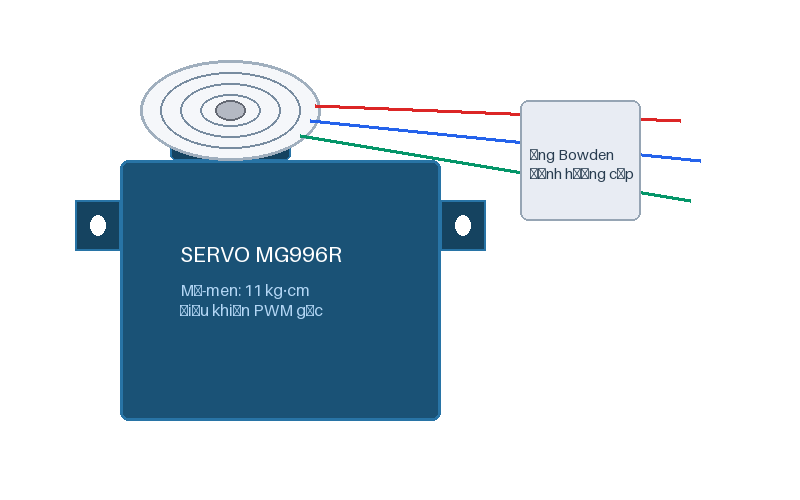
\includegraphics[width=5.0cm, height=2.2cm, keepaspectratio]{assets/servo_spool_assembly.png}
    };
    \node[below=2pt of img_servo, font=\footnotesize] {Cụm 3 Động cơ Servo MG996R \& Tang cuốn cáp};

    \draw[arrowLine] (-1.2, 0) -- (-0.2, 0);

    % Khung cơ cấu Bowden
    \node[innerDashed, text width=4.5cm] (b_bowden) at (2.3, 0) {
      {\bfseries\small Cơ cấu truyền động Bowden}\\[3pt]
      {\scriptsize $\bullet$ Cáp Dyneema kéo gập độc lập}\\[2pt]
      {\scriptsize $\bullet$ Servo nhả cáp chiều duỗi}\\[2pt]
      {\scriptsize $\bullet$ Nẹp đàn hồi hồi vị mu tay}
    };

    % Nhãn bên phải
    \node[anchor=west, align=left, font=\scriptsize] at (4.9, 0) {
      $\bullet$ Cửa sổ thăm dò nỗ lực\\
      $\bullet$ Không cản trở chuyển động\\
      $\bullet$ Giới hạn an toàn hành trình
    };
  \end{tikzpicture}
};

% ==================== TẦNG 4: TẦNG THỊ GIÁC & TÁC VỤ ====================
\node[dashedContainer, text width=15.0cm, below=28pt of t3] (t4) {
  \begin{tikzpicture}
    \node[anchor=west, font=\bfseries\normalsize] at (-7.2, 1.4) {Tầng thị giác đón trước \& Tác vụ (Vision Pre-Actuation Tier)};
    
    % Hình Camera & Depth Anything V2
    \node (img_vis) at (-3.2, 0) {
      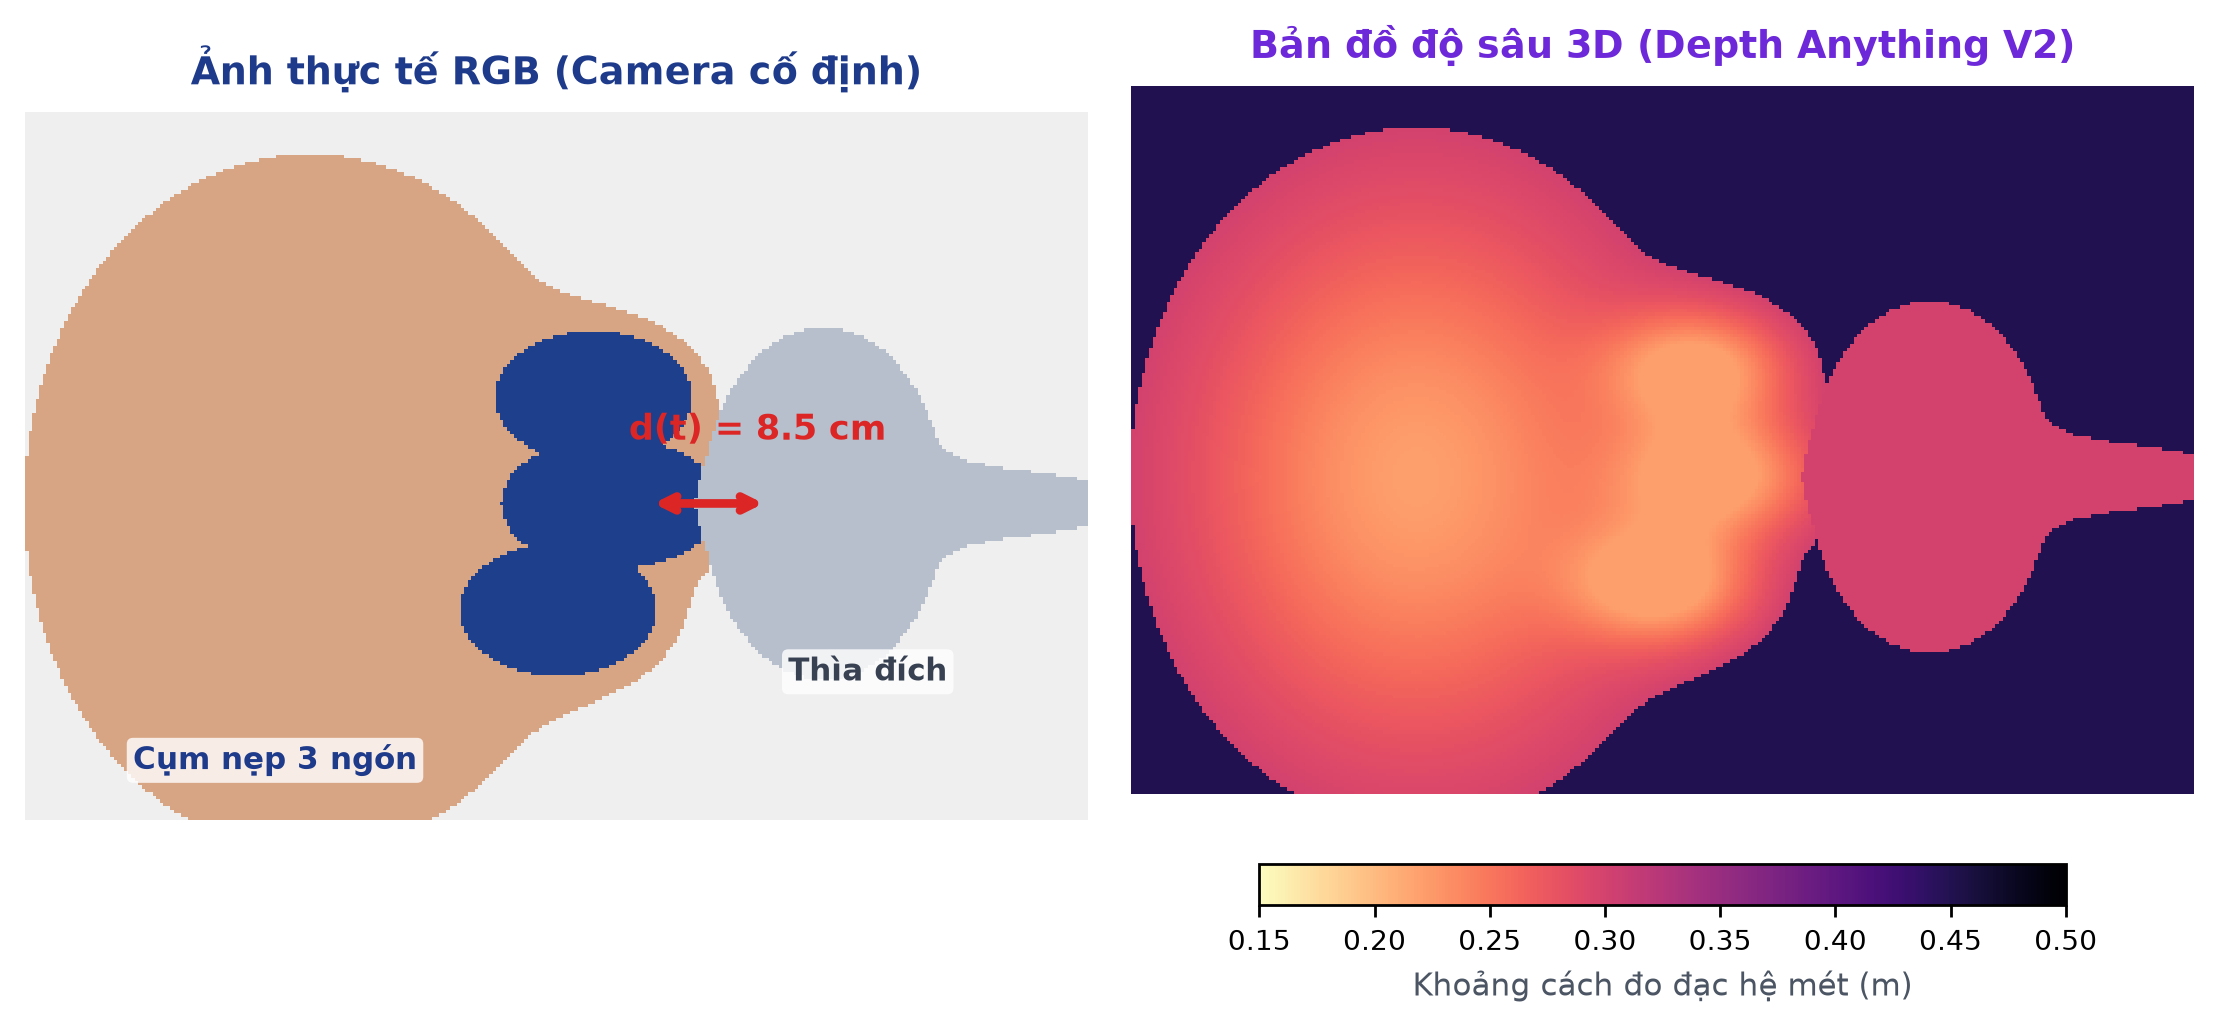
\includegraphics[width=6.6cm, height=2.3cm, keepaspectratio]{assets/depth_anything_scene.png}
    };
    \node[below=2pt of img_vis, font=\footnotesize] {Camera RGB + Bản đồ độ sâu 3D (Depth Anything V2)};

    \draw[arrowLine] (0.5, 0) -- (1.5, 0);

    % Khung tác vụ Orange Pi
    \node[innerDashed, text width=4.5cm] (b_opi) at (4.0, 0) {
      {\bfseries\small Orange Pi 5 Pro (NPU)}\\[3pt]
      {\scriptsize $\bullet$ Đo cự ly 3D tay -- thìa $d(t)$}\\[2pt]
      {\scriptsize $\bullet$ Tính thời gian tới tiếp xúc TTC}\\[2pt]
      {\scriptsize $\bullet$ Đánh giá bài tập kẹp 3 chấu}
    };
  \end{tikzpicture}
};

% ==================== MŨI TÊN LIÊN KẾT GIỮA CÁC TẦNG ====================
\draw[arrowLine] (t1.south) -- node[tagText] {Tín hiệu tương tự 21 kênh (Lực vi sai \& Góc gập)} (t2.north);
\draw[arrowLine] (t2.south) -- node[tagText] {Lệnh điều khiển Servo AAN (Kéo gập / Nhả duỗi)} (t3.north);
\draw[biArrowLine] (t3.south) -- node[tagText] {Trạng thái vận động $\longleftrightarrow$ Cự ly 3D \& Định thời TTC đón trước} (t4.north);

\end{tikzpicture}
\end{document}
